%%% MATERIALS AND METHODS %%%


Put materials and methods used here.

\subsection*{Carbon Fiber Filament}

test text\\

\subsection*{Extruder Design}

test text\\

\subsection*{Finite Element Analysis}

ANSYS Composite PrepPost (ACP) finite element analysis software was used to predict the mechanical properties and failure behavior of the bridge specimen. ACP utilizes orthopic shell elements, ply thickness assignments, oriented element sets, and stackup configurations to model and analyze fiberous, composite structures of multiple layers. Various failure criteria, such as Puck or Tsai-Wu failure theories, are utilized in solving to predict failure modes and critical layers given the applied loads and boundary conditions.

\begin{figure}[htp]
%\centering
\includegraphics[width=0.3\textwidth]{./figures/fea/fea-surface-geometry}
\caption{The surface geometry used in ACP.}
\label{fig:fea-bridge-speciment}
\end{figure}

%test text. test citations \cite{Puck-Stuttgard,Puck-NASA}.\\

\subsection*{Print Controls}

Typical FDM 3D printers, including industrial, home, and do-it-yourself printers, use a Cartesian-style gantry system with 3 degrees of freedom. Such printers can achieve some degree of curved-layer printing, but the fixed print head attitude limits the curved-layer geometries to those accessible from one approach angle. To remove this limitation, a 6-degree-of-freedom FANUC LR Mate 200iC robotic arm was used for this project. The robot provides a similar resolution and repeatibility to other FDM printers, with a somewhat larger build envelope, making it a good candidate to become an FDM printer platform. Some of the remaining elements of the printer control system were chosen from existing open-source hardware and software from the RepRap community, while others were chosen from FANUC products.

Figure~\ref{fig:sys-overview} gives a schematic overview of the mechanical, hardware, and software components that make up the curved-layer 3D printer system. The robot arm is the mechanical platform for the 3D printer. The custom extruder is fitted to the end of the robot arm and acts as a printing end effector. The motion of the robot arm is controlled by the robot controller, which is programmed by writing TP programs via the controller teach pendant. The extruder hardware, including the heater cartridge, cooling fan, and extrusion motor are controlled by an open-source Megatronics board loaded with the (also open-source) Marlin firmware. 

\begin{figure}[t]
    \centering
    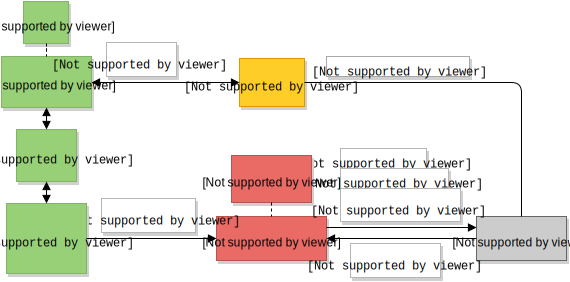
\includegraphics[width=.8\linewidth]{figures/diagrams/system overview}
    \caption{Overview of the 3D printer controls.}
    \label{fig:sys-overview}
\end{figure}

\subsection*{FANUC Setup}

test text\\
